\documentclass[letterpaper, reqno,11pt]{article}
\usepackage[margin=1.0in]{geometry}
\usepackage{color,latexsym,amsmath,amssymb,graphicx,float,listings,tikz}
\usepackage{hyperref}

\hypersetup{
colorlinks=true,
linkcolor=magenta,
filecolor=magenta,
urlcolor=cyan,
}

\graphicspath{ {images/} }

\begin{document}
\pagenumbering{arabic}
\title{Math 318 Homework 3}
\date{03/02/23}
\author{Xander Naumenko}
\maketitle

{\medskip\noindent\bf Question 1a.} Clearly $P(X=x)=0\forall x<4$ since it takes at least 4 games for the game to end. For the remaining games, fix the number of games x and consider the games as repeated Bernoulli trials. There are two possible cases: A won or B won (where the event $A$ is A winning and the event $B$ is B winning). Regardless of which one, the winner must have won the last game (otherwise the game would have ended earlier). The remaining games are distributed in a binomial distribution. Therefore:

\[
    P(X=x\cap A)={x-1\choose 3}p^{4}(1-p)^{x-4}
.\]
\[
    P(X=x\cap B)={x-1\choose 3}p^{x-4}(1-p)^{4}
.\]

Since these are independent events their probability can be summed, so
\[
P(X=x)={x-1\choose 3}p^{4}(1-p)^{x-4}+{x-1\choose 3}p^{x-4}(1-p)^{4}
.\]

{\medskip\noindent\bf Question 1b.} If $X=4$ then clearly A or B won all four games, A winning occurs with probability 
\[
P=\frac{p^{4}}{p^{4}+(1-p)^{4}}
.\]

% {\medskip\noindent\bf Question c.} This is equivalent to finding the probability that after 6 games the two teams are exactly tied, and then A winning the game after that. To find the probability that it's tied after the first 6 games we can use the binomial distribution: 
% \[
%     P(\text{Tied at 6 games})={6\choose 3}p^{3}(1-p)^{3}
% .\]
% To find the total probability of A winning then is just this times the chance that they win 

{\medskip\noindent\bf Question 1c.} To get to the point that $7$ games are played it must have been tied 3-3 previously or else the game would already have been over. The probability that A wins from that point is just the probability that $A$ wins the last game, which is just $P=p$. 


{\medskip\noindent\bf Question 2a.} Let $y$ be the number of unique results. There are ${6\choose y}$ combinations of $y$ numbers that are unique, while there are $6^{4}$ possible combinations of rolls. The number of unique ways of ordering the rolls depend on what $y$ is. 

If $y=1$ then there's only one way of arranging them, and if $y=4$ then there's 4! orderings of rolls. If $y=3$ then ${4\choose 2}3!$ ways of arranging the rolls, since one pair of rolls must result in the same number and there are $3!$ ways of choosing which number has the pair. Finally if $y=2$ then either the rolls are distributed with 2 in each repeated number or there are 3 in 1 and 1 in the other. If it's 2-2 then there are ${4\choose 2}$ ways of arranging the rolls, with 4 choices for the first pair and the remaining in the second. If it's arrange 3-1 there are $2\cdot {4\choose 1}=8$ ways of this occurring. Putting this together: 
\[
    P(Y=1)=\frac{{6\choose 1}1^{4}}{6^{4}}=\frac{1}{216}
.\]
\[
    P(Y=2)=\frac{{6\choose 2}\left( {4\choose 2}+2\cdot 4 \right) }{6^{4}}=\frac{35}{216}
.\]
\[
    P(Y=3)=\frac{{6\choose 3}{4\choose 2}3! }{6^{4}}=\frac{5}{9}
.\]
\[
    P(Y=4)=\frac{{6\choose 4}4! }{6^{4}}=\frac{5}{18}
.\]

The expected value is just the sum of the mass function: 
\[
EY=\sum_{i=1}^{4}i P(Y=i)=\frac{1}{216}+\frac{70}{216}+\frac{15}{9}+\frac{20}{18}\approx 3.1
.\]

{\medskip\noindent\bf Question 2b.} Consider that the probability that the minimum is $z$ is the probability that all the numbers are $z$ or greater minus the probability that they are all $z+1$ or greater. Thus we have: 
\[
P(Z=z)=1-\frac{(6-z)^{4}}{6^{4}}-\left( 1-\frac{(7-z)^{4}}{6^{4}} \right) =\frac{(7-z)^{4}-(6-z)^{4}}{6^{4}}
.\]
For the expected value, again we can just sum over the possibilities: 
\[
EZ=\sum_{i=1}^{4}i P(Z=i)=\sum_{i=1}^{4}\frac{(7-i)^{4}-(6-i)^{4}}{6^{4}}=\frac{2275}{1296}\approx 1.76
.\]

{\medskip\noindent\bf Question 3a.} Summing over the possible outcomes: 
\[
P(Y>m)=\sum_{i=m+1}^{\infty}p(1-p)^{i-i}=p(1-p)^{m}\sum_{i=0}^{\infty}(1-p)^{i}=(1-p)^{m}
.\]

{\medskip\noindent\bf Question 3b.} Computing the limit: 
\[
\lim_{\delta\to 0}\left( 1-\lambda\delta \right)^{\frac{t}{\delta}}
.\]
Let $\delta'=-\delta\lambda$. Then: 
\[
\lim_{\delta'\to 0}\left( 1+\delta' \right)^{-\lambda\frac{t}{\delta'}}
.\]
This is a well known identity for $e$, so it converges to $e^{-\lambda t}$

{\medskip\noindent\bf Question 3c.} From the previous parts, we know that $P(Y>m)$ is approximately an exponential random variable. We also have: 
\[
P(Y>m)=\int_m^{\infty}P(Y=y)dy\implies \frac{d}{dt}(1-e^{-\lambda t})=P(Y=y)\implies P(Y=y)=\lambda e^{-\lambda t}
.\]

{\medskip\noindent\bf Question 4.} Suppose without loss of generality that a 0 is being transmitted (the same argument in reverse works in that case). The probability that the message is received correctly is the probability that the normal distribution is less than $\frac{1}{2}$. Plugging this into a calculator (since the CDF of the normal distribution isn't elementary): 
\[
P=P(N(0,0.04)<0.5)=0.9938
.\]

{\medskip\noindent\bf Question 5a.} The probability mass function of the poisson distribution is $\frac{\lambda e^{-\lambda}}{k!}$. Plugging in $k=2$ and maximizing:
\[
    \frac{d}{d\lambda}\left( \frac{\lambda ^2e^{-\lambda}}{2} \right) =\lambda e^{-\lambda}-\frac{1}{2}\lambda^2e^{-\lambda}=0\implies \lambda=2 
.\]

{\medskip\noindent\bf Question 5b.} $\lambda$ is the mean time between murders, and the average over each week in this case was $1.5$. Thus the $\lambda$ that maximizes the probability of this sequence occurring is $\lambda=1.5$. 

{\medskip\noindent\bf Question 5c.} Again, $\lambda$ is the mean time between murders. This time if we calculate the average time between murders we have to average over the sum of the sequence, so we get: 
\[
\lambda = \frac{1}{k}\sum_{i=1}^{k}a_k
.\]

{\medskip\noindent\bf Question 6a.} 

\begin{lstlisting}[language=Python]
from math import comb

p = 1/50
seats = 420
sold = 430

Prob = 0
for i in range(seats+1,sold+1):
    Prob += p**(sold-i)*(1-p)**i*comb(sold,i)
\end{lstlisting}

\[
\implies P=0.6405
.\]

{\medskip\noindent\bf Question 6b.} 

\begin{lstlisting}[language=Python]
from math import exp,factorial

p = 1/50
seats = 420
sold = 430

lam = p*sold
Prob = 0
for i in range(sold-seats):
    Prob += lam**i*exp(-lam)/factorial(i)

print(Prob)
\end{lstlisting}

\[
\implies P=0.63995
.\]

{\medskip\noindent\bf Question 6c.} 

\begin{lstlisting}[language=Python]
import matplotlib.pyplot as plt 
import numpy as np
from random import randint
from scipy.stats import poisson

p = 1/50
seats = 420
sold = 430
n = 50000

no_shows = []

X = np.arange(1, 30, 1)
Y = poisson.pmf(X, mu=sold*p)

for _ in range(n):
    no_shows.append(sum(randint(1,50)==1 for _ in range(sold)))

plt.hist(no_shows, density=True, bins=24)
plt.plot(X,Y)
plt.show()
\end{lstlisting}

\begin{figure}[htpb]
    \centering
    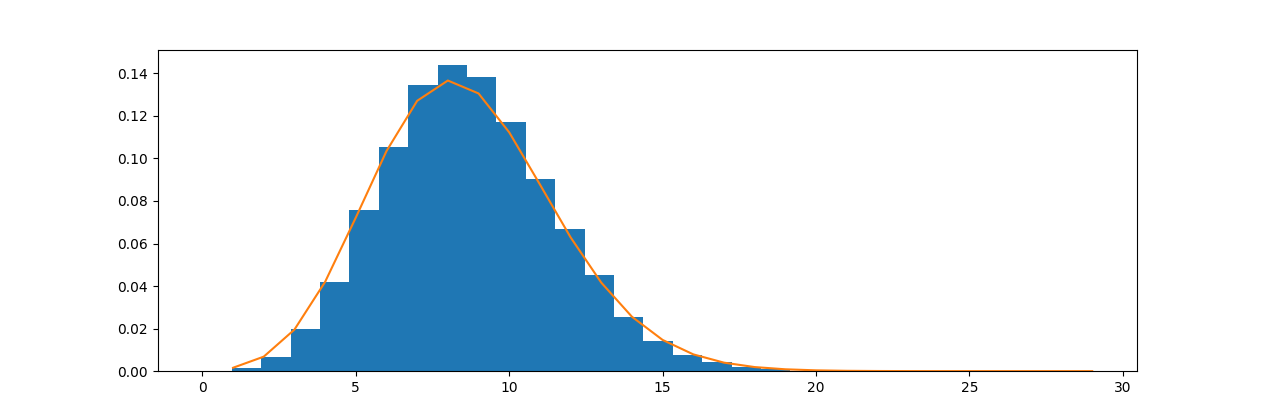
\includegraphics[width=0.8\textwidth]{c}
    \caption{Graph for question c}
    \label{fig:c}
\end{figure}

{\medskip\noindent\bf Question 6d.} As can be seen by figure \ref{fig:d}, the series eventually stabalizes to approximately 0.65. This means that the airline in the long run expect around 65\% of flights to be overbooked. 

\begin{lstlisting}[language=Python]
import matplotlib.pyplot as plt 
import numpy as np
from random import randint
from scipy.stats import poisson

p = 1/50
seats = 420
sold = 430
n = 50000

no_shows = []

for _ in range(n):
    no_shows.append(sum(randint(1,50)==1 for _ in range(sold)))

N = np.arange(1,n+1,1)
Xn = []
tot = 0
for i in range(len(no_shows)):
    tot += no_shows[i] < sold-seats
    Xn.append(tot / (i+1))

print(Xn[-1])
plt.plot(N,Xn)
plt.show()
\end{lstlisting}


\begin{figure}[htpb]
    \centering
    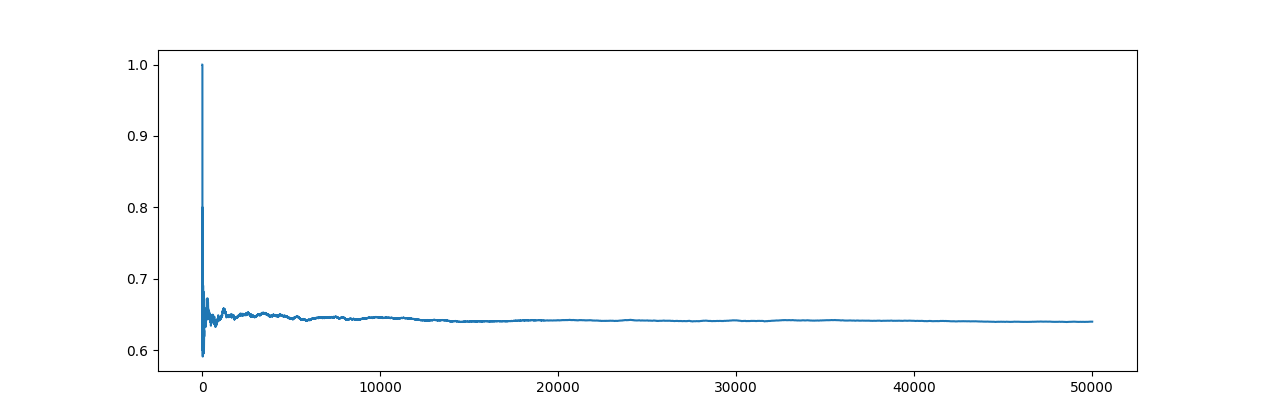
\includegraphics[width=0.8\textwidth]{d}
    \caption{Graph for part d}
    \label{fig:d}
\end{figure}

% We'll do it last minute, like we always do. It'll be super successful, just like it never is -Nader Kamali


\end{document}
